\title{\huge{Neural Information Retrieval}}
\author{
		David Guaty Domínguez C512 
		\and
		Adrián Rodríguez Portales C512 
	    \and  Rodrigo D. Pino Trueba C512 }
\date{June 2022}

\documentclass[12pt]{article}
\usepackage{amsmath}
\usepackage{amsfonts} 
\usepackage{csquotes}
\usepackage{hyperref}
\usepackage{listings}
\usepackage{graphicx}

\begin{document}
\maketitle


% \providecommand{\keywords}[1]
% {
%     \small
%     \textbf{\textit{Keywords---}} #1 
% }

% \keywords{aprendizaje profundo, sistema de recuperación de información,redes neuronales}


\section{Introducción}

A lo largo de la historia de la humanidad,  el proceso de  almacenar y recuperar la información ha sido una tarea 
bastante difundida. Sin embargo con el surgimiento de Internet y del \textit{Big Data}, los volúmenes de información 
actuales son cada vez más grandes y se hace necesario el surgimiento de herramientas más sofisticadas 
para poder satisfacer estas 
necesidades. El estudio de esta área se le conoce como Recuperación de Información ( \textit{Information Retrieval} ).
Entre los modelos clásicos utilizados se encuentran el booleano y el vectorial. Ambos modelos presentan ventajas en 
determinadas situaciones, pero en muchos escenarios no logran cumplir con los requerimientos del sistema. 

La aparición del aprendizaje automático (\textit{machine learning}) y ,en especial, del aprendizaje profundo
(\textit{deep learning}), ha permitido revolucionar la industria y la ciencia . 
Los sistemas de recuperación de información no se han quedado atrás. El enfoque conocido como \textit{Learning to Rank} 
\cite{learningtorank} usa técnicas de aprendizaje automático para la tarea de recuperar información. Existen 
tres formas principales de resolver este problema:

\begin{itemize}
	\item \textit{pointwise}: Este enfoque es el más sencillo de implementar y fue el primero en proponerse para las
		tareas de \textit{Learning to Rank}.
	\item \textit{pairwise}: El problema con el enfoque anterior es que se necesita la relevancia absoluta de un documento
		con respecto a una consulta. Sin embargo, en muchos escenarios esta información no estás disponible, entonces lo
		que se puede saber es, por ejemplo, que documento tiene mayor relevancia de una lista según la selección de un usuario 
	\item \textit{listwise}: Este enfoque es el más difícil, pero también el más directo. A diferencia de los dos anteriores
		, donde el problema se reduce a una regresión o clasificación, este trata de resolver el problema de ordenación
		directamente.
\end{itemize}

Dentro de los modelos de aprendizaje automático más usados recientemente para el proceso de \textit{ranking}, se encuentran las redes neuronales. A la aplicación de este conjunto de técnicas en la recuperación de información se le 
conoce como \textit{Neural Information Retrieval} \cite{mitra2018an}. En este trabajo usaremos este enfoque y compararemos los resultados
con un modelo de recuperación de información clásico ( vectorial ).


\section{Diseño del sistema de recuperación de información}

TODO: Hablar un poco de la arquitectura general de la aplicación

\subsection{Preprocesamiento de los datos}

Los dataset utilizados fueron preprocesados para obtener aquellas
palabras que tienen mayor semántica. Durante este proceso se
realizaron dos tareas:

\begin{itemize}
	\item Eliminación de \textit{stopwords}:los \textit{stopwords} son
		términos muy comunes que brindan poca información semántica
		en un texto o documento. Generalmente suelen ser adverbios,
		pronombres y artículos.
	\item \textit{Lemmatization}: este proceso consiste en llevar a las
		palabras a su raíz gramatical, haciendo análisis morfológico 
		de los términos y eliminando cualquier inflexión. Esto permite
		indexar términos con igual semántica como uno solo .
\end{itemize}

Ambas tareas se hicieron con la biblioteca de Python \textit{Spacy}

\subsection{Modelo vectorial}

El modelo vectorial\cite{vectormodel} es un modelo algebraico que representa los documentos
y la consulta como vectores con pesos. Cada término indexado representa
una dimensión del vector, por lo que el vocabulario del corpus es
quien define la dimensión del espacio vectorial.

Para el cálculo de los pesos existen varias formas. Una de las más 
usadas es \textit{tf-idf}. Esta tiene entre sus ventajas que es 
fácil de computar. Sin embargo, como está basado en el modelo
\textit{bag of words}, no tiene en cuenta el orden de las palabras
en el texto.

Para calcular el \textit{tf} se utilizó la siguiente fórmula:

$$tf_{ij} = K + \frac{(1-K)freq_{ij}}{\max_{i} freq_{ij}}$$

En el caso del \textit{idf} se utilizó:

$$idf_i= \log \frac{N}{n_i}$$

donde $N$ es el total de documentos en el corpus y $n_i$ es la
cantidad de documentos donde aparece el término $i$. Luego con estos 
valores los pesos se obtenían como $w_{ij}= tf_{ij}*idf_{ij}$.

Finalmente para obtener la similitud entre la consulta y los 
documentos se usó el coseno del ángulo :

$$sim(d_{j},q) = \frac{ d_{j} \cdot q }{ |d_{j}||q| }$$


\subsection{Modelo con redes neuronales}

Para determinar qué tan relevante es un documento para una consulta dada se implementaron modelos de redes neuronales. En total, en la aplicación existen cuatro de estos modelos. 

La función del modelo de red neuronal es determinar, para una consulta $q$ y un documento $d$, un ranking $N(q,d)$, donde $N$ es la red neuronal. Este valor de ranking varía de acuerdo al conjunto de datos con el cual el modelo se entrenó. Por ejemplo, en el conjunto de datos \textit{Cranfield} existen los niveles de relevancias $\{-1,1,2,3,4\}$, los cuales se mapearon a $\{0,1,2,3,4\}$. Un valor de relevancia $0$ significa que el documento $d$ es totalmente irrelevante a la consulta $q$ y un valor de relevancia de $4$ significa que el documento es una total respuesta a la consulta por el usuario.

Entonces se tienen un conjunto de datos de entrenamiento que tiene la forma $(documento, consulta, relevancia)$, es el trabajo de la red neuronal aprender estas relaciones.

Los cuatros modelos son:
\begin{itemize}
	\item Un clasificador y un regresor mediante redes convolucionales
	\item Un clasificador y un regresor mediante redes recurrentes con capas LSTM
\end{itemize}

Investigaciones recientes han empleado redes neuronales convolucionales o redes neuronales recurrentes para la clasificación de textos motivados por el notable éxito del aprendizaje profundo \cite{wu2017convolutional}.


Para la implementaci\'on de los modelo se utiliz\'o keras debido a sus facilidades para el preprocesamiento de texto y para elaborar arquitecturas de manera sencilla.

Para cada uno de lo tipos de redes, las arquitecturas del clasificador y el regresor son en esencia las mismas; el cambio fundamental es en la capa de salida y en la funci\'on de p\'erdida.

Dicho esto se explica la arquitectura general seguida para la red convolucional:
\begin{itemize}
	\item Capa de Embedding: Para representar los vectores de documento y consulta en un espacio vectorial continuo de dimensi\'on fija peque\~na. Esto es \'util pues aumenta el rendimiento con respecto al procesamiento de lenguaje natural y puede capturar algo de la sem\'antica de la palabra. Para el embedding se us\'o un modelo preentrenado: GloVe. Mediante glove se puede obtener la matriz de la capa del embedding de la red.
	
	 \begin{lstlisting}[frame=single, breaklines, language=Python] 
embeddings_index = {}
with open(path_to_glove_file) as f:
	for line in f:
		word, coefs = line.split(maxsplit=1)
		coefs = np.fromstring(coefs, "f", sep=" ")
		embeddings_index[word] = coefs
	print("Found %s word vectors." % len(embeddings_index))
	 
	 \end{lstlisting}
	
	\item Capa de convoluci\'on
	\item Capa(s) densamente conectadas
	\item Capa de salida
\end{itemize}

En c\'odigo, generalmente el modelo convolucional es de la siguiente manera:
	 \begin{lstlisting}[frame=single, breaklines, language=Python] 
input_doc = keras.Input(shape=(None,), dtype="int64")
input_query = keras.Input(shape=(None,), dtype="int64")

embedding_layer = Embedding( #GloVe
	num_tokens,
	embedding_dim,
	embeddings_initializer=keras.initializers.Constant(embedding_matrix),
	trainable=False,
)

embedded_sequences = embedding_layer(input_doc)
x = layers.Conv1D(128, 5, activation="relu")(embedded_sequences)
x = layers.GlobalMaxPooling1D()(x)


embedded_sequences = embedding_layer(input_query)
y = layers.Conv1D(128, 5, activation="relu")(embedded_sequences)
y = layers.GlobalMaxPooling1D()(y)

combined = layers.Concatenate()([x, y])

# Para clasificador
z = layers.Dense(16, activation="relu")(combined)
z = layers.Dense(number_of_relevance_levels, activation="softmax")(z)

#Para regresor
z = layers.Dense(16, activation="relu")(combined)
z = layers.Dense(1)(z) 

\end{lstlisting}

La arquitectura de la red recurrente tiene la siguiente forma:
\begin{itemize}
	\item Una capa de Embedding, anteriormente mencionada.
	\item Una capa LSTM bidireccional:  Esta capa propaga su entrada hacia adelante y hacia atrás y luego concatena la salida final.
	\item Capas densamente conectadas: Después de que la capa anterior haya convertido la secuencia en un solo vector, estas capas realizan un procesamiento final y convierten esta representación vectorial en un solo logit como salida de clasificación o regresi\'on.
\end{itemize}

En c\'odigo, generalmente el modelo recurrente es de la siguiente manera:
\begin{lstlisting}[frame=single, breaklines, language=Python] 
embedding = tf.keras.layers.Embedding(
  input_dim=len(encoder.get_vocabulary()),
  output_dim=64,
  mask_zero=True,
) 

input_doc = keras.Input(shape=(None,), dtype="int64")
input_query = keras.Input(shape=(None,), dtype="int64"

doc_embedding = embedding(input_doc)
query_embedding = embedding(input_query)

doc_bid = tf.keras.layers.Bidirectional(
  tf.keras.layers.LSTM(64, return_sequences=True)
)(doc_embedding)

query_bid = tf.keras.layers.Bidirectional(
  tf.keras.layers.LSTM(64, return_sequences=True)
)(query_embedding)

x = keras.layers.Concatenate()([doc_bid, query_bid])

x = tf.keras.layers.Dense(64, activation="relu")(x)
x = tf.keras.layers.Dropout(0.5)(x)

output = keras.layers.Dense(1)(x)
\end{lstlisting}

\subsection{Ventajas y desventajas de las redes neuronales}
 
 A menudo, es posible realizar un entrenamiento de extremo a extremo en aprendizaje profundo para una aplicación, lo que quiere decir que se pueden dise\~nar modelos cuya entrada sea el texto en lenguaje natural introducido por el usuario. Esto se debe a que estos modelos ofrecen una rica representabilidad y la información en los datos se puede codificar de manera efectiva en el modelo.
 
 Como ventajas de las redes neuronales para el procesamiento de texto se tiene:
 \begin{itemize}
 	\item Puede reconocer patrones en el texto
 	\item Puede aprender representaciones del texto, como por ejemplo los embedding mencionado
 	\item Mejora su rendimiento cuanto m\'as datos existan
 	\item Captura mejor la sem\'antica del texto que otros m\'etodos
 \end{itemize}

En las tareas de procesamiento de texto mediante redes neuronales existe una falta de fundamento teórico, as\'i como falta de interpretabilidad del modelo y el requisito de una gran cantidad de datos y recursos computacionales potentes.

Como desventajas se tienen:

\begin{itemize}
	\item Se requiere grandes cantidades de datos para ser entrenadas
	\item Dependiente de hardware en su eficiencia para entrenarse
	\item Los modelo de redes neuronales son cajas negras dif\'iciles de analizar
	\item Si el conjunto de entrenamiento no esta bien depurado pueden producirse errores en el aprendizaje y no generalizar como se quiere
\end{itemize}

\subsection{Problemas encontrados en entrenamiento}

Al entrenar las redes neuronales mediante el conjunto de datos de Cranfield se encontr\'o con el problema del overfitting. Los modelos aprenden muy bien el conjunto de entrenamiento pero tienen bajos rendimiento en el conjunto de validaci\'on. En la figura 1 se puede observar el diagn\'ostico del entrenamiento de la red y como se produce el overfitting.

Para tratar de solucionar este problema se intent\'o:
\begin{itemize}
	\item Simplificar el modelo poniendo menos capas intermedias y con menos neuronas
	\item A\~nadir capas de Dropout
	\item Para el entrenamiento cuando las dos curvas mostradas en la figura 1 empiezan a divergir
	\item Cambiar la funci\'on de activaci\'on en las capas intermedias
	\item Aumentar la dimensi\'on del embedding
\end{itemize}

Lamentablemente ninguna de estas v\'ias solucion\'o el problema del overfitting, por lo que es recomendable usar otro conjunto de datos como corpus para entrenar los modelos.

\begin{figure}
	\centering
	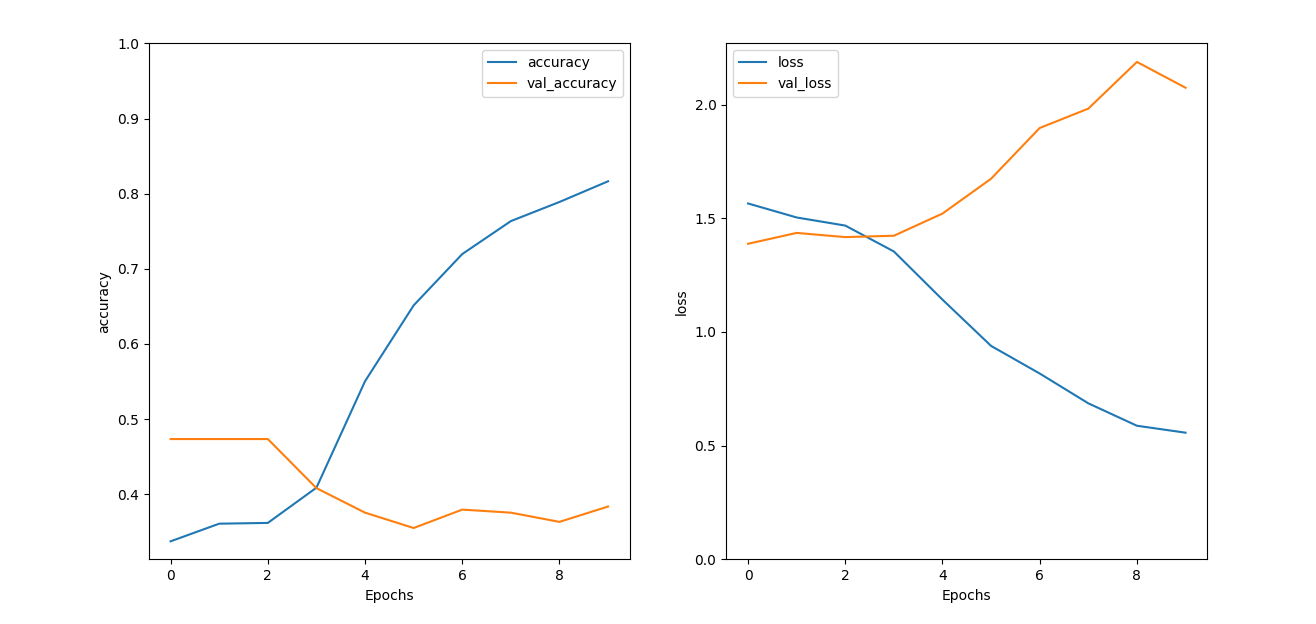
\includegraphics[width=0.7\linewidth]{img/overf}
	\caption{Overfitting encontrado en entrenamiento}
	\label{fig:overf}
\end{figure}



\section{Análisis de los resultados} 


\section{Conclusiones} % recomendaciones en esta sección también

En este trabajo se implement\'o un sistema conocido como \textit{Learning To Rank} en el cual se usan redes neuronales para predecir la relevancia que tiene un documento dada una consulta del usuario. Tratar de hallar la relevancia para todos los documentos del corpus mediante la red neuronal es muy costoso, por lo que se implement\'o un modelo vectorial que da un conjunto de documentos sobre los cuales la red neuronal halla las relevancias. En el entrenamiento de las redes neuronales se encontr\'o el problema del overfitting el cual no pudo ser resuelto por las t\'ecnicas intentadas.

Se recomienda la b\'usqueda de mas conjuntos de entrenamiento que tengan mayor cantidad de datos y analizar si se produce overfitting en estos casos. Tambi\'en se podr\'ian implementar otras arquitecturas de redes neuronales, como por ejemplo Transformers.



% \nocite{*}
\bibliographystyle{abbrv}
\bibliography{simple}

\end{document}
